\section{方法框架}

% Page: IA-DR 总体框架
\begin{frame}{\algoNotation{} 总体框架}
\begin{columns}[T,totalwidth=\textwidth]
\column{0.5\textwidth}
\begin{center}
\includegraphics[width=\linewidth]{../figure/algo/main.pdf}
\end{center}

\column{0.48\textwidth}
\begin{block}{四个核心组件}
\small
\begin{enumerate}
    \item<1-> \hl{超级行程表示}：压缩行程空间，构造吸引力上界
    \item<2-> \hl{聚合下界模型}：在聚合网络上给出有效下界
    \item<2-> \hl{完整网络上界修复}：频率固定 + 超级行程收入约束 $\to$ 可行解
    \item<3-> \hl{可实现性检验}：必要时添加时间点，保证收敛
\end{enumerate}
\end{block}
\end{columns}
%% Overlay annotations (3-step animation)
\begin{tikzpicture}[remember picture, overlay]
  \only<1>{\node[red, font=\small\bfseries, anchor=west] at ([xshift=-3.5cm,yshift=-1.2cm]current page.east) {$\leftarrow$ 核心贡献};}
  \only<2>{\node[red, font=\small\bfseries, anchor=west] at ([xshift=-3.5cm,yshift=-2.5cm]current page.east) {$\leftarrow$ 形成双侧界};}
  \only<3>{\node[red, font=\small\bfseries, anchor=west] at ([xshift=-6.5cm,yshift=-3.5cm]current page.east) {$\leftarrow$ 保证算法最优并收敛};}
\end{tikzpicture}
\end{frame}


% Page: 超级行程表示
\begin{frame}{核心概念——超级行程表示}
\begin{columns}[T,totalwidth=\textwidth]
\column{0.55\textwidth}
\begin{block}{路径签名与分组}
\[r \eqRelByPathSig r' \;\Longleftrightarrow\; \pathSig{r}=\pathSig{r'}\]
\small
相同\hl{聚合路径签名}的原始行程归并为一个超级行程 $R$。
\end{block}

\vspace{0.2cm}
\begin{block}{超级行程的作用}
\begin{itemize}
    \item 压缩原始行程变量规模
    \item 保留顾客选择中的收入结构
    \item 吸引力上界\hl{抑制不可实现收入}
\end{itemize}
\end{block}

\column{0.4\textwidth}
\begin{center}
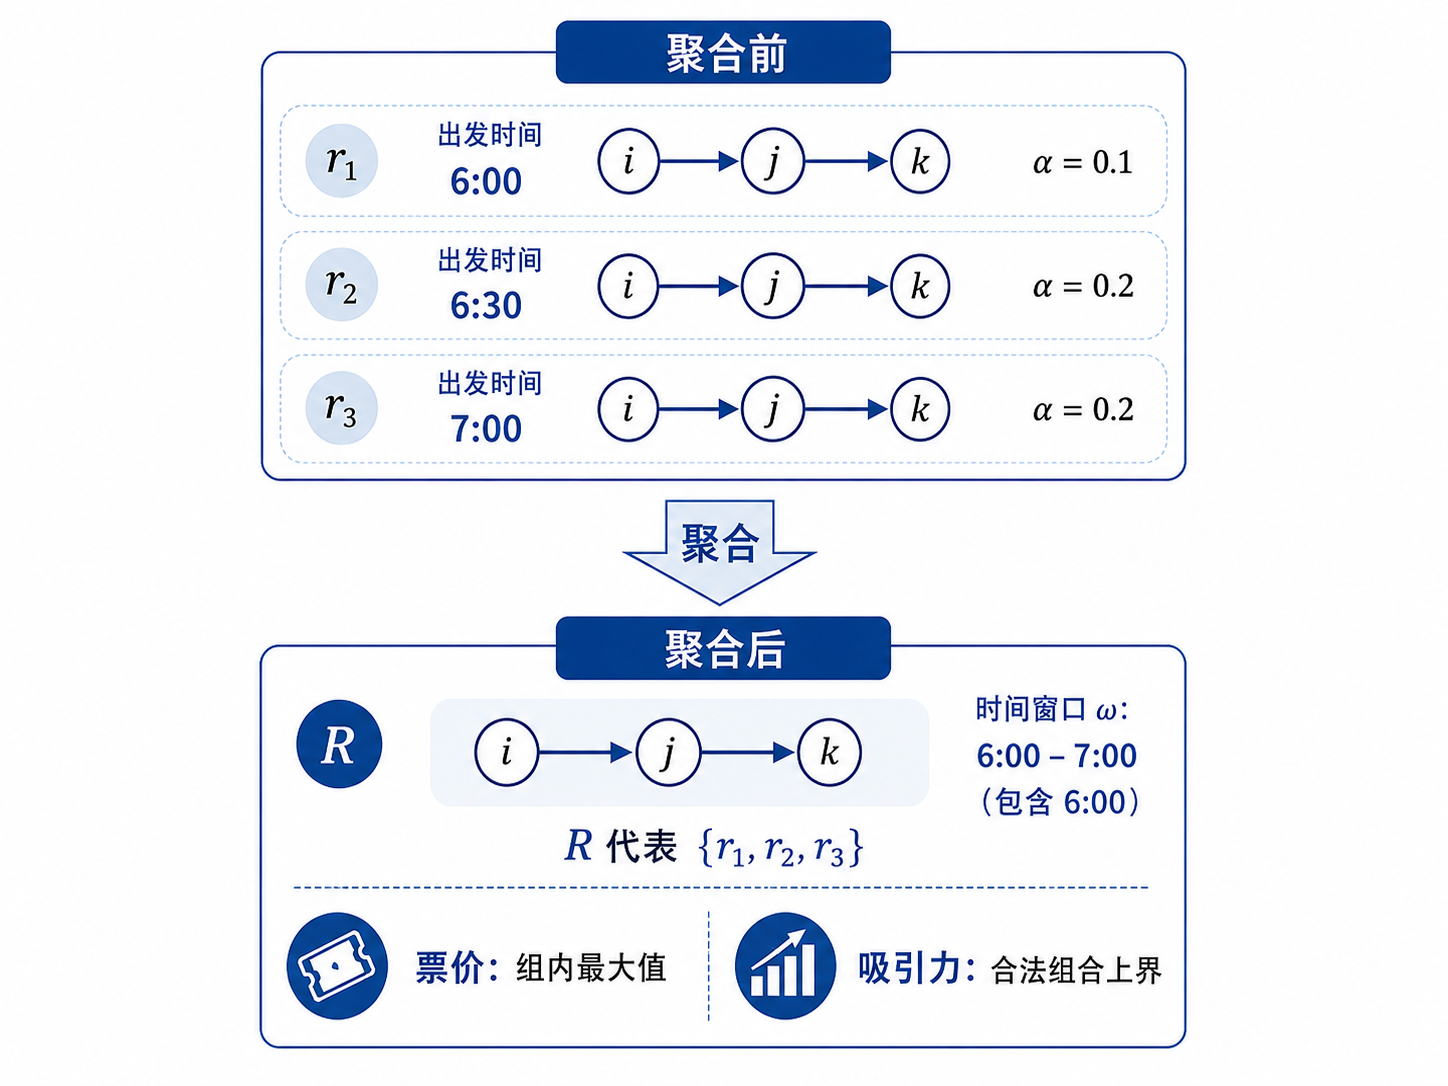
\includegraphics[width=\linewidth]{figure/iti_agg.png}
\end{center}
\end{columns}
\end{frame}


% Page: 双侧界模型
\begin{frame}{双侧界模型：下界与上界}
\begin{columns}[T,totalwidth=\textwidth]
\column{0.48\textwidth}
\begin{block}{聚合下界模型}
\begin{itemize}
    \item 聚合时空网络（粗离散化）
    \item 超级行程空间（压缩行程变量）
    \item 吸引力上界约束
\end{itemize}
\vspace{0.2cm}
\centering
$\Downarrow$\\[3pt]
\hl{有效下界}
\end{block}

\column{0.48\textwidth}
\begin{block}{完整网络上界修复}
\begin{itemize}
    \item 完整时空网络（原始离散化）
    \item 频率固定（锁定下界解的服务频率）
    \item 收入上界约束
\end{itemize}
\vspace{0.2cm}
\centering
$\Downarrow$\\[3pt]
\hl{原问题可行解}（上界）
\end{block}
\end{columns}

\vspace{0.4cm}
\centering
\small 下界评价理论最优水平，上界来自真实可行解，二者差距即\hl{最优性间隙}。
\end{frame}


% Page: 可实现性检验与收敛
\begin{frame}{松弛解可实现性检验}
\begin{block}{核心思想}
\begin{itemize}
    \item 聚合松弛解可能在完整网络中不可实现
    \item 检测到非法情形后，添加对应时间点
    \item 更新路径签名与超级行程划分，缩小松弛间隙
\end{itemize}
\end{block}

\vspace{0.4cm}
\begin{alertblock}{理论保证}
算法在有限步内闭合上下界；实际计算中以预设最优性容差停止。
\end{alertblock}
\end{frame}
